\documentclass[conference]{IEEEtran}
\IEEEoverridecommandlockouts
% The preceding line is only needed to identify funding in the first footnote. If that is unneeded, please comment it out.
\usepackage[colorlinks=true, linkcolor=blue, urlcolor=blue, citecolor=blue, anchorcolor=blue]{hyperref}
% \usepackage{cite}
\usepackage{amsmath,amssymb,amsfonts}
\usepackage{algorithmic}
\usepackage{graphicx}
\let\oldincludegraphics\includegraphics
\renewcommand{\includegraphics}[1]{\oldincludegraphics[width=0.5\textwidth,keepaspectratio]{#1}}
\usepackage{textcomp}
% \usepackage[mathletters]{ucs}
\usepackage[utf8]{inputenc}
\usepackage[T1]{fontenc}
\DeclareUnicodeCharacter{0301}{\'e}

\usepackage[normalem]{ulem}
% Avoid problems with \sout in headers with hyperref
\pdfstringdefDisableCommands{\renewcommand{\sout}{}}
\usepackage[style=ieee,backend=bibtex]{biblatex}
\bibliography{ass1.bib}

\providecommand{\tightlist}{%
  \setlength{\itemsep}{0pt}\setlength{\parskip}{0pt}
}

\def\BibTeX{{\rm B\kern-.05em{\sc i\kern-.025em b}\kern-.08em
    T\kern-.1667em\lower.7ex\hbox{E}\kern-.125emX}}
\begin{document}

\title{Scalable Algorithms and Systems for Big Data\\
% {\footnotesize \textsuperscript{*}Note: Sub-titles are not captured in Xplore and should not be used}
% \thanks{Identify applicable funding agency here. If none, delete this.}
}

\author{\IEEEauthorblockN{Stone Fang (Student ID: 19049045)}
\IEEEauthorblockA{\textit{Computers and Information Sciences} \\
\textit{Auckland University of Technology}\\
Auckland, New Zealand \\
fnk7060@autuni.ac.nz}}

\maketitle

\begin{abstract}

In recent years, enormous data is being produced at increasing speed,
posing new challenges to traditional database and data processing
technologies. As a response, a variety of big data technologies have
emerged and are still evolving. To gain an overview and also in-depth
knowledge of scalable data analysis methodologies, this report reviews
three important areas in this topic. First, scalable data indexing plays
a key role in distributed data retrieval and computing optimisation.
Second, big data infrastructure, including storage and computational
framework, is the foundation of all applications. Third, data mining and
machine learning algorithms should be parallelised in order to make the
most of big data. Though great efforts have been put into this area,
there are still open issues such as big data in decentralised computing
environment and multimedia big data analytics.

\end{abstract}

\begin{IEEEkeywords}
big data, distributed computing, scalability, data mining, machine learning
\end{IEEEkeywords}

\hypertarget{introduction}{%
\section{Introduction}\label{introduction}}

In recent years, huge volumes of data have been generated by a variety
of sources such as e-businesses, communications, mobile phones, social
media sites, web servers, sensor networks, cameras, banks, stock
markets, and so on \autocite{OUSSOUS2018431,SIVARAJAH2017}. Nowadays,
data are being generated at an unprecedented rate, bringing us into an
era of big data or ``data deluge'' \autocite{SIVARAJAH2017,hu2014}. The
types of data vary from text to multimedia including image, audio and
video, and the format can be structured, semi-structured and
unstructured. In fact, more than 90\% of the overall data generated in
the real world are unstructured \autocite{SIVARAJAH2017}.

Big data bears enormous potential values with the expectation of
transforming the humans society, and is consequently regarded as the
``new oil'' by some researchers \autocite{hu2014}. It does not only
bring large amount of revenues to businesses and values to consumers,
but also have great potential applications in a range of industries. For
instance, health or medical data analysis has many advantages including
personalised health service, disease evolution monitoring, and adaptive
public health plans \autocite{OUSSOUS2018431}. Another example is the
real-time analysis of data generated by smart meters, sensors and
control devices on smart grid, which can help in incident detection,
risk identification, and energy consumption forecast
\autocite{OUSSOUS2018431}. In commercial environment, companies such as
Google, Amazon, Facebook and Twitter have been greatly benefited from
big data techniques and applications \autocite{Hewage2018}.

Before the big data revolution, it is difficult to store, manage or
analyse datasets in large volumes because of the limited store capacity
and lack of scalability, flexibility and performance in traditional
technologies \autocite{OUSSOUS2018431}. Relational database management
system (RDBMS), the main technology in traditional data management, does
not fit the requirements of big data analysis. The reasons of this
mismatch are mainly twofold, that is:

\begin{itemize}
\tightlist
\item
  Data structure: RDBMS only supports structured data, while has little
  capability in storage and analysis of semi-structured and unstructured
  data \autocite{hu2014}.
\item
  Scalability: RDBMS only scales up at high costs of hardware, and is
  very difficult to scale out, which makes it incapable in continuously
  growing data scenarios \autocite{hu2014,SIVARAJAH2017}.
\end{itemize}

\begin{figure}
\hypertarget{fig:compare}{%
\centering
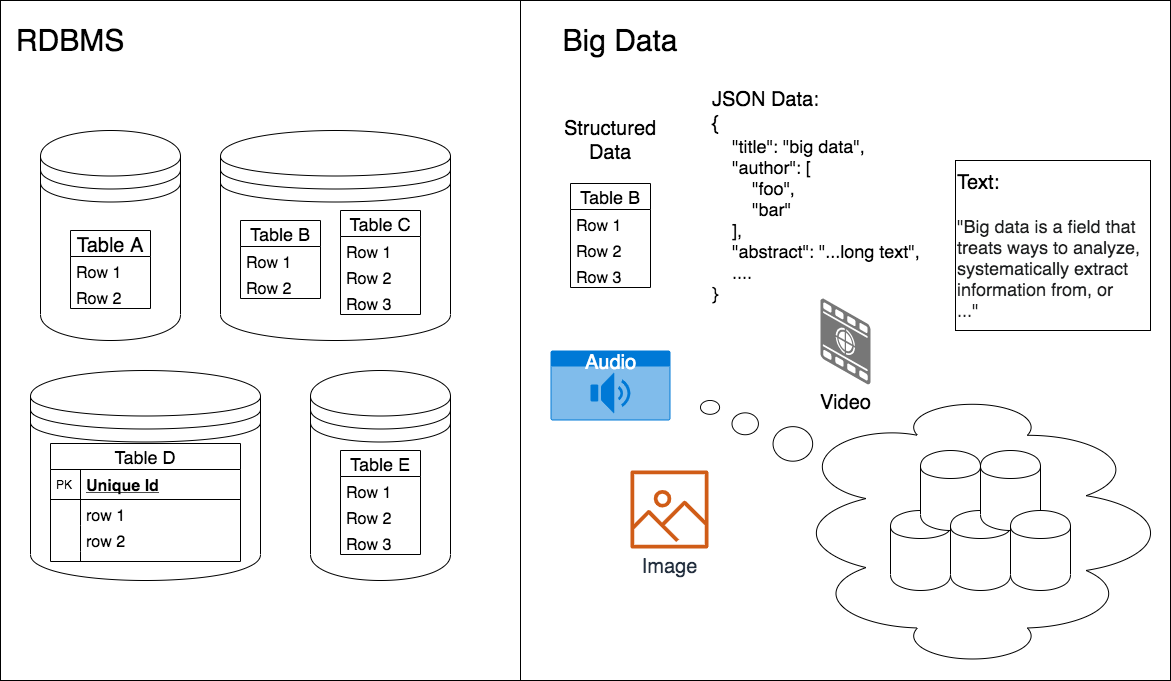
\includegraphics{img/big-data-rdbms.png}
\caption{Comparison between RDBMS and Big Data}\label{fig:compare}
}
\end{figure}

A demonstration of difference between traditional RDBMS and big data
technology is shown in Fig. \ref{fig:compare} .

As a response to the big values and big challenges inside big data,
interests from both academia and industry are dramatically increasing in
recent years. A wide range of issues have been studied at different
levels including data storage, cleaning, analysis, visualisation, and so
on, some of them still open to research \autocite{OUSSOUS2018431}. In
the industry, many companies have their own big data platforms, for
example, Google's large data storage Google File System(GFS) and cloud
based data management system Fusion Table \autocite{Hewage2018}. Many
big data systems and platforms including open-source ones have been
being developed, for instance, NoSQL Databases, BigQuery, MapReduce,
Hadoop, HiveQL, Spark, to mention but a few
\autocite{Hewage2018,SIVARAJAH2017,hu2014}. Some projects have also been
launched by governments of countries such as USA and Japan to catch big
data opportunities \autocite{OUSSOUS2018431}.

\hypertarget{background}{%
\section{Background}\label{background}}

The main characteristics of big data are described as three Vs, namely
Volume, Velocity and Variety \autocite{OUSSOUS2018431,hu2014}. First of
all, the large volume of data is an essential difference between big
data and traditional data \autocite{hu2014}. Second, the velocity at
which the data are being generated implies that the processing and
analysis of datasets should be carried out at a comparable rate to the
data production \autocite{hu2014}. Third, big data are produced in
various format including text and multimedia from various data sources,
resulting in high heterogeneity and diversity
\autocite{OUSSOUS2018431,Pouyanfar2018}. In addition to these three Vs,
some researchers add ``Value'' to extend to a four Vs model
\autocite{hashem_rise_2015}.

There are many types of data that big data analysis systems need to cope
with. Web data is a common one important for search engines such as
Google. Amazon has its shopping and transaction data, and Facebook and
Twitter have a huge number of social media data including user profile
and posts. Log file is also an important type of data that is generated
by web service companies especially cloud-computing providers
\autocite{hu2014}. Wireless sensor networks is another important source
of data, generating a variety of sensor data including sound, force,
temperature, pressure, chemical, and so on \autocite{hu2014}.
Bioinformatics is another area benefited from big data analytics. For
instance, a DNA sequence analysis system was built and deployed in the
Amazon cloud, and another one for biological molecular analysis was
constructed on top of Hadoop \autocite{hashem_rise_2015}. Big data also
advances some science areas which generates massive volume of data such
as high energy physics and astronomy.

According to a well-accepted system engineering methodology in industry,
the big data value chain is decomposed into four consecutive stages
\autocite{hu2014}:

\begin{itemize}
\tightlist
\item
  \textbf{Data generation} refers to the processes that data are
  generated from various sources.
\item
  \textbf{Data acquisition} focuses on the obtaining and collection of
  data.
\item
  \textbf{Data storage} concerns the persistent data storage and
  effective data management.
\item
  \textbf{Data analytics} is the stage concerning the extraction of
  value from data by exploring, transforming, modelling and visualising
  data with analytical tools.
\end{itemize}

The mismatch between the requirements of big data and existing data
management hardware and software platforms raises many challenges to
both industry and research community. Many researches and practices,
especially relating to the scalability, have been conducted among the
four phases, including:

\begin{itemize}
\tightlist
\item
  Network architectures and protocols with high throughput, low latency
  and optimal energy consumption for large-scale data transmission
  \autocite{hu2014}
\item
  Scalable data cleaning, aggregation and duplication removal method for
  huge dataset at reasonable speed but still with acceptable accuracy.
  It is essential for big data quality and reliability
  \autocite{hu2014,OUSSOUS2018431}
\item
  Infrastructures, file systems and database technologies for
  distributed and scalable data storage. More specific issues include
  data partitioning and replication scheme, scalable data indexing and
  query, CAP option (consistency, availability and partition tolerance),
  concurrency control mechanism, parallel and distributed programming
  model \autocite{hu2014,Gupta2016}.
\item
  Scalable machine learning on large dataset, including deep learning on
  large dataset, online (or stream) learning, parallel reinforcement
  learning, computational framework for machine learning, and so on
  \autocite{OUSSOUS2018431,Gupta2016}
\item
  Real-time or near real-time analysis of large increasing volume of
  data \autocite{OUSSOUS2018431}
\item
  Imbalanced big data analysis \autocite{OUSSOUS2018431}
\item
  Big data visualisation \autocite{hu2014}
\end{itemize}

Given so many challenges in big data, this report will conduct dive
deeper into detailed studies on the following themes: 1) big data
indexing and retrieval; 2) big data infrastructure; 3) scalable data
mining and machine learning.

\hypertarget{literature-review}{%
\section{Literature Review}\label{literature-review}}

\hypertarget{big-data-indexing}{%
\subsection{Big Data Indexing}\label{big-data-indexing}}

While the volume of data is growing explosively and unstructured
contents are gaining dramatically increasing weight in the overall data,
existing data indexing strategies, mainly designed for RDBMS, do not
satisfies the requirement for efficient retrieval and querying of huge
amount of heterogeneous data\autocite{gani2016,Pouyanfar2018}. As a
result, many indexing algorithms have been proposed as responses to this
challenge. In general, indexing strategies can be put into three
categories: non-Artificial Intelligence (NAI), Artificial Intelligence
(AI), and Collaborative Artificial Intelligence (CAI) approaches
\autocite{gani2016,Pouyanfar2018}.

NAI approaches include tree-based (B\textsuperscript{+}-tree, R-tree and
X-tree), bitmap-based and hash-based methods \autocite{gani2016}.
\textcite{lu2014} proposed ScalaGiST, a scalable generalised search
tree, for distributed data indexing working seamlessly with the
open-source MapReduce system of Hadoop. It can be easily implemented
with widely-used B\textsuperscript{+}-tree and R-tree, and supports not
only conventional query but also multi-dimensional range and similarity
queries. The author also demonstrated the dynamic deployment to large
Hadoop clusters to cope with large number of users and huge volume of
data \autocite{lu2014}.

\textcite{ma2017} proposed an in-memory distributed indexing method
benefited from Apache Spark system for large-scale media data searching.
The author created feature vectors for each data, and built M-trees for
indexing on each computing node. The local indexing method is claimed to
be replaceable by any other tree-based or hash-based indexing structure.
Over 30x speed-up was gained by this system in the experiments.

\textcite{xie2019} proposed a novel indexing approach, called
COordinate-based INdexing (COIN), for data sharing in edge computing
environment. Unlike the mainly master/slave-architectured cloud
computing systems, edge computing ones are working in a more
peer-to-peer way. COIN models the network topology in a virtual
2-dimensional (2-D) coordinate system, maps a data index into this 2-D
space by a hash function, and forwards a data index to an edge node
closest to the coordinate of this data index. The experiments on a real
network and simulation on large-scale network showed that COIN has
shorter average path length and less number of forwarding entries than
the DHT method which has been widely studied and applied in real world
distributed systems.

\textcite{Wang_2016} conducted a comprehensive survey on hash-based big
data indexing methods with learnable hash functions. Locality Sensitive
Hashing (LSH) refers to a specific kind of hashing methods which are
more likely to generate closer hash codes (that is, more bits are the
same) of two data points if they have higher similarity in the original
space, which is consequently an ideal method for approximate nearest
neighbour (ANN) search. The hash function can be data-dependent, which
is adjusted to the target data by machine learning algorithms to
maximise the indexing performance. For example, some algorithms such as
Spectral Hashing learns hash functions to make the data more balanced.

\hypertarget{big-data-infrastructures}{%
\subsection{Big Data Infrastructures}\label{big-data-infrastructures}}

Big data infrastructures such as MapReduce and Spark play important role
in scalable big data analysis because it handles the intensive and
repetitive underlying works such as data distribution, replication,
resource allocation and fault-tolerance for programmers
\autocite{Gupta2016}. A large number of big data infrastructures,
usually including distributed file system (DFS), database and
computational frameworks, have been proposed and developed in industrial
settings by open-source foundations and companies such as Amazon,
Facebook, Google, Twitter, and so forth \autocite{Gupta2016,Hewage2018}.

\hypertarget{distributed-file-system}{%
\subsubsection{Distributed File System}\label{distributed-file-system}}

DFS provides scalable and reliable data storage via distribution and
replication of data blocks across a collection of interconnected
machines \autocite{Gupta2016}. As an successful example in industry,
Google developed its DFS solution named Google File System (GFS), the
largest DFS cluster in the world \autocite{Hewage2018}. Other companies
also developed own cloud-based big data storage, such as Microsoft's
Azure and Amazon's S3 \autocite{hashem_rise_2015}. There are also
several open-source solutions for DFS, among which HDFS is the most
widely used one, and Ceph, GlusterFS and XtreemFS are some other
alternatives \autocite{Gupta2016}.

\hypertarget{data-model}{%
\subsubsection{Data Model}\label{data-model}}

Novel data models and database technologies are required for big data
due to the lack of scalability of traditional RDBMS
\autocite{Gupta2016}. Two main categories of big data models are Not
Only SQL (NoSQL) and NewSQL.

\hypertarget{nosql}{%
\paragraph{NoSQL}\label{nosql}}

While RDBMS rigorously complies with ACID principle (Atomicity,
Consistence, Isolation, Durability), NoSQL databases focus on horizontal
scalability and availability, and comply with BASE properties (Basically
Available, Soft-state, Eventually consistent) \autocite{Gupta2016}.
There are four categories of NoSQL models which is adopted by a variety
of researches
\autocite{grolinger_data_2013,hashem_rise_2015,Gupta2016,hu2014}:

\begin{itemize}
\tightlist
\item
  Key-value store: In such a system, data are stored as values
  associated with keys, and can be accessed only by exact match with
  keys, which resembles a dictionary or associative map. It is
  appropriate for fast equality query, for example, retrieving user
  profile by its ID. For example, Amazon builds its own key-value
  storage system Dynamo \autocite{Hewage2018}. Some other typical
  systems are Memcached, Redis, Voldemort, BerkeleyDB, and Riak
  \autocite{grolinger_data_2013}.
\item
  Column-family store: It stores data in a column-oriented structure
  which is similar to rational databases. However, unlike RDBMS, it
  stores data in distributed manner and does not require pre-defined
  table schema. It is pioneered by Google's BigTable which eventually
  becomes an ancestor of most other column-family store systems. HBase
  as part of Hadoop ecosystem is an open-source implementation of
  BigTable concepts. Some other well-known systems includes Facebook's
  Cassandra and Amazon's SimpleDB and DynamoDB
  \autocite{grolinger_data_2013,hu2014}.
\item
  Document-oriented store: These systems model data as documents in some
  kind of standard data exchange format, most of them JSON (JavaScript
  Object Notation) or its variations \autocite{grolinger_data_2013}.
  Different documents do not necessarily contain the same attributes,
  thus providing a schema-free storage. Some representatives are CouchDB
  and MongoDB \autocite{Gupta2016}.
\item
  Graph database: It stores data as graphs containing vertices (or
  nodes) and edges (or links) with associated properties, thus is
  suitable for data with extensive interconnections
  \autocite{grolinger_data_2013}. Some typical systems are Neo4j,
  InfoGrid, and GraphDB \autocite{Gupta2016}.
\end{itemize}

\hypertarget{newsql}{%
\paragraph{NewSQL}\label{newsql}}

NewSQL is an alternative of big data models, also known as next
generation solutions for scalable RDBMS, which combines the advantages
of both RDBMS and NoSQL. Specifically, it provides the scalability of
NoSQL systems without sacrificing the ACID properties of rational
databases \autocite{Gupta2016}. Some representatives are NuoDB and
VoltDB \autocite{Gupta2016}. Spanner, developed by Google, is seen as a
NewSQL database over the cluster distributed globally
\autocite{grolinger_data_2013,hu2014}. F1, also by Google and build upon
Spanner, implements many RDBMS-like features such as strict schema along
with high scalability such as dynamic sharding and consistent
replication. It is backing Google's advertisement business
\autocite{hu2014}.

\hypertarget{distributed-computational-framework}{%
\subsubsection{Distributed Computational
Framework}\label{distributed-computational-framework}}

Computational framework is another important part of big data
infrastructure, which can be categorised into three modes: batch mode,
real-time, and hybrid mode \autocite{Gupta2016}.

\hypertarget{batch-mode}{%
\paragraph{Batch Mode}\label{batch-mode}}

In batch mode, data to be proceeded are divided into batches which are
computed in parallel across a cluster of nodes. The most well-known
batch mode distributed processing framework is MapReduce, which
basically consists of map and reduce stages
\autocite{hashem_rise_2015,Gupta2016}. However, each MapReduce iteration
has to load data from disk and write it back into disk, causing
significant deficiency in executing iterative computational tasks. As a
result, it is losing popularity in recent years \autocite{Gupta2016}.
Hadoop is an open-source implementation of MapReduce along with other
facilities such as its DFS, HDFS.

\hypertarget{real-time-mode}{%
\paragraph{Real-Time Mode}\label{real-time-mode}}

In real-time processing mode, data are modelled as streams, that is,
processed immediately on its arrival. One of the most well-known stream
processing system is Storm, which models the computation as a graph of
spouts and bolts \autocite{Gupta2016}. Some alternatives are Trident and
S4 \autocite{Gupta2016,hu2014}.

\hypertarget{hybrid-model}{%
\paragraph{Hybrid Model}\label{hybrid-model}}

Hybrid model is, as its name suggests, a unified framework for both
batch and real-time processing \autocite{Gupta2016}. Spark is the most
widely used hybrid framework. The basic building block of Spark is
Resilient Distributed Dataset (RDD), with the major advantage of
in-memory computation which greatly reduced the disk I/O operation.
Spark also provides micro-batch streaming for real-time processing, in
which the incoming stream data is divided into small chunks
\autocite{Gupta2016}. The core of Spark is general engine that models
computational tasks into DAGs able to handle different type of workloads
such as batch processing, streaming, SQL-like query and graph analytics
\autocite{hashem_rise_2015}.

\hypertarget{lambda-architecture}{%
\subsubsection{Lambda Architecture}\label{lambda-architecture}}

All models have their own pros and cons. Lambda architecture is a
unified architecture with a set of principles for big data
infrastructure design. It decomposes the overall system into three
layers, namely batch, speed, and serving. The batch layer hold immutable
data in its storage by appending new data on arrival, and produces batch
view in batch mode. The speed layer executes real-time computation on
new data to compensate the latency in batch layer. Finally the outputs
of batch layer and speed layer are merged into serving layer for query
\autocite{Gupta2016}.

\hypertarget{scalable-data-mining-and-machine-learning}{%
\subsection{Scalable Data Mining and Machine
Learning}\label{scalable-data-mining-and-machine-learning}}

Traditional data mining and machine learning algorithms usually work
with data fully loaded into memory at a central point, which is not
suitable for distributed computing systems. As a response, parallel or
distributed algorithms have been intensively studied and implemented
\autocite{gan2017,Gupta2016}. \textcite{gan2017} conducted a
comprehensive survey on a number of distributed data mining algorithms
in five categorise, including frequent itemset mining, frequent sequence
mining, frequent graph mining, clustering, and privacy issues in
distributed data mining. This survey includes not only the algorithms
based on MapReduce or Spark framework, but also those applicable to
general distributed systems such as P2P systems and ad hoc networks
\autocite{gan2017}. In another survey, \textcite{Gupta2016} reviewed,
summarised and categorised a variety of researches on parallel machine
learning algorithms, including unsupervised learning (such as K-means,
density-based clustering, hierarchical clustering, spectral clustering),
supervised learning (such as decision tree, Fuzzy Rule-Based
Classification System, Naive Bayes, Support Vector Machine),
semi-supervised learning (such as cotraining, active learning),
reinforcement learning (such as Markov Decision Process, Q-Learning),
and deep learning. Most of them are based on MapReduce or Spark
framework. Moreover, the author analysed the optimisation tactics that
could improve the performance of distributed algorithms mostly by
reducing disk I/O and/or network communication overhead, as well as
metrics used for evaluating the performance against their serial
counterparts. It is also worth noticing that the accuracy may decrease
due to data distribution, leaving a trade-off between accuracy and
speedup \autocite{Gupta2016}.

\hypertarget{discussionopinion}{%
\section{Discussion/Opinion}\label{discussionopinion}}

As large amount of data are being produced at a rapid increasing speed,
new ideas and technologies are emerging among data processing and
analytics. This is still a fast developing area with a number of
challenges and opportunities.

\hypertarget{big-data-indexing-1}{%
\subsection{Big Data Indexing}\label{big-data-indexing-1}}

Data indexing is a fundamental and essential operation for any big data
applications. Efficient indices can significantly reduce the amount of
data that needs to be retrieved in a computational task, which is even
more important in distributed environments such as MapReduce.
Considering that more and more big data applications are moving onto
some kind of distributed computing infrastructure such as cloud
computing platform, distributed data indexing has been rising in
importance. Most indexing strategies are either tree-based or
hash-based, with open issues remaining. As the size of data center
grows, existing algorithms decrease in performance on clusters with
thousands of machines. Moreover, with the rising of edge computing with
numerous edge devices such as mobile phones and sensor nodes, indexing
methods for cloud-based architecture become less efficient. Therefore,
we need the data distribution and indexing to be more balanced and
distinguishable over the cluster. Another problem could be indexing
multimedia data such as image and video. To cope with this problem, we
need more intelligent methods, for example, incorporation of machine
learning algorithms into hash-based indexing for better representation.

\hypertarget{big-data-infrastructures-1}{%
\subsection{Big Data Infrastructures}\label{big-data-infrastructures-1}}

Infrastructures including storage, database, computational framework,
distributed resource management play an essential role in big data
technology and applications. These systems usually handles computational
resource management, data consistency, scalability, and many other
issues over clusters of distributed computing nodes.

DFS provides transparent data storage by making a cluster of computers
behave like a single storage machine. It frees end-user from burdens of
data distribution, replication and fault-recovery. Some open-source
solutions such as HDFS and Ceph have been developed for over a decade.
However, there are still some problems. For example, most DFSs employ
master-slave architecture, in which the master nodes are vulnerable and
potential bottleneck when the the cluster are scaled up to thousands of
machines, limiting its maximum cluster size. To improve this, some
methods would be beneficial such as autonomous, robust and efficient
master election algorithms. Another issue is the optimisation of data
distribution and replication to minimise the network transportation on
query or computational jobs.

Database or data model for big data is a key factor and has been
intensively researched and implemented. Nowadays we have different types
of data models and numerous implementations either commercial or
open-sourced. However, this area is still not mature. First, different
models are specialised in certain area, therefore, decisions have to be
made based on the business requirement and usually multiple systems need
to be combined into one integrated system in complex real-world
applications. A more general or unified model can make the technology
selection and combination more efficient and reliable. Second, unlike
the generally-used SQL in RDBMS, different big data databases have their
own query interface. Therefore, a unified or standard query interface
would be beneficial, which can be some SQL-like language or its
extension. However, designing a universal query interface on a variety
of diverse distributed databases remains a challenging question.

Computational frameworks make distributed computing and data processing
easier and faster. Ideally, a distributed computational framework would
hide all the low-level details, and make programming on it without the
awareness of its distributed nature. This requires the framework
sophisticated and able to dynamically optimise the computation based on
the incumbent data and tasks. It also should collaborate with the
underlying storage or database to maximise local computing and minimise
the intercommunication across machines which is the least efficient part
in distributed computational systems. The gap between batch computing
and stream processing is another problem. Though we already have some
unified system such as Spark that can handle both modes, they are quite
different in nature and practice, and even controversial at some time.
Lambda architecture provides a viable approach that split the overall
system into offline and real-time part, but its rather a set of
principles than a model or framework.

\hypertarget{scalable-data-mining-and-machine-learning-1}{%
\subsection{Scalable Data Mining and Machine
Learning}\label{scalable-data-mining-and-machine-learning-1}}

Distributed big data computational frameworks do not automatically
parallelise data mining and machine learning algorithms without extra
effort. In order to utilise the benefits of scalability and speedup of
distributed computing, algorithms need to be carefully re-designed for
parallelism. It is worth noticing that not all algorithms have the same
difficulty in parallelism because of their internal dependencies. For
example, in decision tree a split node can be computed only after its
parented node generated; by contrast, algorithms that can be fit into
the form of matrix multiplication would be parallelised more easily
thanks to the parallel matrix operation. However, random forest is much
wider and less high than decision tree so it would enjoy higher
parallelism. Another issue is the lack of some common framework that can
be widely adapt to the parallelisation of a range of algorithms, so at
this point researchers and engineers have to re-design each individual
algorithm in order to exploit the data mining and machine learning
technologies. Such kind of approach causes redundant work and less
generality. Though there are some existing frameworks that can express
machine learning algorithms into a graph of basic computations at an
abstract level, most of them focus on a sub-area such as Tensorflow for
deep learning. Therefore, a universal framework for algorithm
parallelisation will greatly reduce the workload, and provide consistent
interface for programmers while hides the details of underlying
infrastructure.

\hypertarget{conclusion}{%
\section{Conclusion}\label{conclusion}}

Nowadays enormous amount of data with high variety in nature is being
generated at exponential-growing speed, which is becoming a rising power
that can change the world. However, such large volume of data poses new
challenges to existing data technologies because traditional RDBMS
designed for centralised processing on structured data with well-defined
schema. Therefore, new technologies are demanding to handle a variety of
data including numeric, text, multimedia, graph and others at large and
ever-growing scale. This is a large topic as big data covers a wide
range of areas, which can be roughly divided into four phases,
specifically, data generation, collection, storage and analysis. As it
is impossible to cover every aspect of such as large topic, this report
focuses on three theme, that is, scalable data indexing, big data
infrastructure, and scalable data mining and machine learning
algorithms. Firstly, several data indexing algorithms such as tree-based
and hash-based indexing are reviewed under distributed environment
including cloud computing as well as the emerging edge computing which
usually works in more decentralised and peer-to-peer way. Secondly, big
data infrastructures are summerised and analysed, including distributed
file system, NoSQL and NewSQL databases, and batch and real-time
computational frameworks. A large number of systems are available under
either commercial or open-source licenses, leaving technological
decision-making a tricky task. Thirdly, parallel and distributed data
mining and machine learning algorithms are reviewed, showing that these
algorithms have been being comprehensively studied, but still lack a
unified approach or framework.

\hypertarget{future-issues}{%
\section{Future Issues}\label{future-issues}}

Having been under intensive development for more than a decade, big data
technology is still at an early stage and remains a fast-changing area.
In this report two future issues are stated as follows.

\hypertarget{decentralised-big-data-system}{%
\subsection{Decentralised Big Data
System}\label{decentralised-big-data-system}}

Recent big data systems are mainly based on cloud computing at
geologically centralised data center, but it is not the only case.
Distributed system has several other forms such as grid, peer-to-peer
network, ad hoc networks, social networks, and so forth
\autocite{gan2017}. With the emerging of smartphones and Internet of
Things (IoT), massive amount of data are produced by edge devices. This
trend leads the rising of big data processing in fog computing and edge
computing environment \autocite{singh_fog_2019}, which is, however, a
less studied area. Different from the dominant master-slave architecture
in cloud computing, edge computing systems work in a more decentralised
or peer-to-peer way, which requires different infrastructures other than
the cloud-based ones.

\hypertarget{multimedia-big-data-processing}{%
\subsection{Multimedia Big Data
Processing}\label{multimedia-big-data-processing}}

Large-scale multimedia data processing \autocite{Pouyanfar2018} is
another big challenge and lack of studies. Multimedia such as images and
videos are significantly larger in size than structured data, posing
challenges in the storage system and computational framework. For
example, the significance and difficulty of scalability in multimedia
storage system is escalated by the large volume and variety of data. As
another example, distributed systems utilising a hybrid of CPU and GPU
will greatly speed up multimedia data processing. A more recent area,
multi-modal data mining methods jointly analyse multiple types of data.
For instance, texts, images and videos on social media can be jointly
mined for additional benefits than separated analysis on each individual
type of data.

% \bibliography{ass1}{}
% \bibliographystyle{IEEEtran}

\printbibliography

\end{document}
